\documentclass[border=6pt]{standalone}

% Shared visual language for the standalone PVI--GCNM presentation assets.
% Each asset inputs this file from its tables/, charts/, or galleries/ folder.

\usepackage{amsmath}
\usepackage{graphicx}
\usepackage[table]{xcolor}
\usepackage{array,booktabs,tabularx,multirow}
\usepackage{tikz}
\usetikzlibrary{arrows.meta,calc,patterns,patterns.meta,positioning}
\usepackage{pgfplots}
\pgfplotsset{compat=1.18}

% Tectonic uses optical-size Latin Modern files by default.  Pin the text
% family to the 10pt masters and scale them continuously; this keeps the
% standalone assets renderable from a minimal offline bundle while preserving
% every requested display size.  Other LaTeX engines simply keep their normal
% font setup.
\makeatletter
\ifdefined\UnicodeFontFile
  \IfFileExists{/usr/share/fonts/dejavu-sans-fonts/DejaVuSans.ttf}{%
    \DeclareFontFamily{TU}{assetsans}{}
    \DeclareFontShape{TU}{assetsans}{m}{n}
      {<-> \UnicodeFontFile{/usr/share/fonts/dejavu-sans-fonts/DejaVuSans.ttf}{\UnicodeFontTeXLigatures}}{}
    \DeclareFontShape{TU}{assetsans}{m}{it}
      {<-> \UnicodeFontFile{/usr/share/fonts/dejavu-sans-fonts/DejaVuSans-Oblique.ttf}{\UnicodeFontTeXLigatures}}{}
    \DeclareFontShape{TU}{assetsans}{m}{sl}{<->ssub*assetsans/m/it}{}
    \DeclareFontShape{TU}{assetsans}{bx}{n}
      {<-> \UnicodeFontFile{/usr/share/fonts/dejavu-sans-fonts/DejaVuSans-Bold.ttf}{\UnicodeFontTeXLigatures}}{}
    \DeclareFontShape{TU}{assetsans}{b}{n}{<->ssub*assetsans/bx/n}{}
    \DeclareFontShape{TU}{assetsans}{bx}{it}
      {<-> \UnicodeFontFile{/usr/share/fonts/dejavu-sans-fonts/DejaVuSans-BoldOblique.ttf}{\UnicodeFontTeXLigatures}}{}
    \DeclareFontShape{TU}{assetsans}{b}{it}{<->ssub*assetsans/bx/it}{}
    \DeclareFontFamily{TU}{assetmono}{}
    \DeclareFontShape{TU}{assetmono}{m}{n}
      {<-> \UnicodeFontFile{/usr/share/fonts/urw-base35/NimbusMonoPS-Regular.otf}{\UnicodeFontTeXLigatures}}{}
    \DeclareFontShape{TU}{assetmono}{bx}{n}
      {<-> \UnicodeFontFile{/usr/share/fonts/urw-base35/NimbusMonoPS-Bold.otf}{\UnicodeFontTeXLigatures}}{}
    \DeclareFontShape{TU}{assetmono}{b}{n}{<->ssub*assetmono/bx/n}{}
    \renewcommand{\familydefault}{assetsans}
    \newcommand{\AssetMonoFont}{\fontfamily{assetmono}\selectfont}
  }{%
    \renewcommand{\familydefault}{\sfdefault}
    \newcommand{\AssetMonoFont}{\ttfamily}
  }
  \DeclareFontFamily{TU}{lmr}{}
  \DeclareFontShape{TU}{lmr}{m}{n}
    {<-> \UnicodeFontFile{lmroman10-regular}{\UnicodeFontTeXLigatures}}{}
  \DeclareFontShape{TU}{lmr}{m}{it}
    {<-> \UnicodeFontFile{lmroman10-italic}{\UnicodeFontTeXLigatures}}{}
  \DeclareFontShape{TU}{lmr}{m}{sl}{<->ssub*lmr/m/it}{}
  \DeclareFontShape{TU}{lmr}{m}{sc}{<->ssub*lmr/m/n}{}
  \DeclareFontShape{TU}{lmr}{bx}{n}
    {<-> \UnicodeFontFile{lmroman10-bold}{\UnicodeFontTeXLigatures}}{}
  \DeclareFontShape{TU}{lmr}{b}{n}{<->ssub*lmr/bx/n}{}
  \DeclareFontShape{TU}{lmr}{bx}{it}{<->ssub*lmr/bx/n}{}
  \DeclareFontShape{TU}{lmr}{b}{it}{<->ssub*lmr/bx/n}{}
\else
  \renewcommand{\familydefault}{\sfdefault}
  \newcommand{\AssetMonoFont}{\ttfamily}
\fi
\DeclareFontShape{OT1}{cmr}{m}{n}{<->cmr10}{}
\DeclareFontShape{OT1}{cmr}{m}{it}{<->ssub*cmr/m/n}{}
\DeclareFontShape{OT1}{cmr}{m}{sl}{<->ssub*cmr/m/n}{}
\DeclareFontShape{OT1}{cmr}{bx}{n}{<->cmbx10}{}
\DeclareFontShape{OT1}{cmr}{b}{n}{<->ssub*cmr/bx/n}{}
\DeclareFontShape{OML}{cmm}{m}{it}{<->cmmi10}{}
\DeclareFontShape{OML}{cmm}{b}{it}{<->cmmib10}{}
\DeclareFontShape{OMS}{cmsy}{m}{n}{<->cmsy10}{}
\DeclareFontShape{OMS}{cmsy}{b}{n}{<->ssub*cmsy/m/n}{}
\DeclareFontShape{OMX}{cmex}{m}{n}{<->cmex10}{}
\makeatother

% Meaning-first palette from the asset specification.
\definecolor{srlNavy}{HTML}{141C2E}
\definecolor{baselineGray}{HTML}{8A93A0}
\definecolor{physicsTeal}{HTML}{1D9E75}
\definecolor{learnedBlue}{HTML}{1D5F8A}
\definecolor{oracleAmber}{HTML}{BA7517}
\definecolor{realCoral}{HTML}{D85A30}
\definecolor{backgroundGreen}{HTML}{4C956C}
\definecolor{lightNavy}{HTML}{E9EFF4}
\definecolor{lightGray}{HTML}{F2F4F6}
\definecolor{lightTeal}{HTML}{E5F4EF}
\definecolor{lightCoral}{HTML}{FBECE7}
\definecolor{ruleGray}{HTML}{D6DADE}
% Seven flat bins approximating Matplotlib RdBu_r for conductivity scales.
\definecolor{rdBlueDark}{HTML}{2166AC}
\definecolor{rdBlue}{HTML}{67A9CF}
\definecolor{rdBlueLight}{HTML}{D1E5F0}
\definecolor{rdNeutral}{HTML}{F7F7F7}
\definecolor{rdRedLight}{HTML}{FDDBC7}
\definecolor{rdRed}{HTML}{EF8A62}
\definecolor{rdRedDark}{HTML}{B2182B}

\setlength{\parindent}{0pt}
\setlength{\tabcolsep}{6pt}
\renewcommand{\arraystretch}{1.25}

\newcolumntype{L}[1]{>{\raggedright\arraybackslash}p{#1}}
\newcolumntype{C}[1]{>{\centering\arraybackslash}p{#1}}
\newcolumntype{R}[1]{>{\raggedleft\arraybackslash}p{#1}}
\newcolumntype{Y}{>{\raggedright\arraybackslash}X}

% No authentic logo file was present in the checked repositories.  Redefine
% \SRLLogo before \input if the deck's official mark becomes available.
\providecommand{\SRLLogo}{%
  \tikz[baseline=(mark.base)]\node[
    draw=srlNavy, line width=0.5pt, inner xsep=4pt, inner ysep=2pt,
    text=srlNavy, font=\AssetMonoFont\bfseries\normalsize
  ] (mark) {SRL};%
}

\newcommand{\AssetTitle}[1]{%
  \noindent\begin{minipage}{\linewidth}
    {\color{srlNavy}\rule{\linewidth}{1.8pt}}\par\vspace{4pt}
    \begin{tabularx}{\linewidth}{@{}>{\raggedright\arraybackslash}X r@{}}
      {\color{srlNavy}\fontsize{25}{29}\selectfont\mdseries #1} & \SRLLogo
    \end{tabularx}
  \end{minipage}%
}

\newcommand{\AssetCaption}[1]{%
  \noindent\begin{minipage}{\linewidth}
    \color{srlNavy}\small\textbf{Takeaway.}\enspace #1
  \end{minipage}%
}

\newcommand{\TaskLine}[1]{%
  \noindent\begin{tikzpicture}
    \node[
      fill=lightNavy, text=srlNavy, anchor=north west,
      inner xsep=7pt, inner ysep=6pt, text width=\dimexpr\linewidth-16pt\relax,
      align=left, font=\small
    ] at (0,0) {#1};
  \end{tikzpicture}%
}

\newcommand{\PseudoTag}[1]{%
  \noindent\begin{tikzpicture}
    \node[
      fill=lightCoral, draw=realCoral, line width=0.6pt,
      text=realCoral, anchor=north west, inner xsep=7pt, inner ysep=6pt,
      text width=\dimexpr\linewidth-16pt\relax, align=left,
      font=\AssetMonoFont\bfseries\normalsize
    ] at (0,0) {#1};
  \end{tikzpicture}%
}

\newcommand{\SyntheticTag}[1]{%
  \noindent\begin{tikzpicture}
    \node[
      fill=lightNavy, draw=learnedBlue, line width=0.6pt,
      text=learnedBlue, anchor=north west, inner xsep=7pt, inner ysep=5pt,
      text width=\dimexpr\linewidth-16pt\relax, align=left,
      font=\AssetMonoFont\bfseries\normalsize
    ] at (0,0) {#1};
  \end{tikzpicture}%
}

\newcommand{\MetricUp}{\,$\uparrow$}
\newcommand{\MetricDown}{\,$\downarrow$}
\newcommand{\Winner}[1]{\textbf{#1}}

% A non-decorative, flat-binned conductivity key. Arguments are
% caption, negative endpoint, and positive endpoint.
\newcommand{\DivergingScale}[3]{%
  \begin{tikzpicture}[baseline=(scaleLabel.base),x=0.42cm,y=0.28cm]
    \foreach \x/\c in {0/rdBlueDark,1/rdBlue,2/rdBlueLight,3/rdNeutral,
                         4/rdRedLight,5/rdRed,6/rdRedDark}{
      \fill[\c] (\x,0) rectangle ++(1,1);
    }
    \draw[srlNavy,line width=0.4pt] (0,0) rectangle (7,1);
    \node[anchor=east,font=\scriptsize,text=srlNavy] at (-0.15,0.5) {#2};
    \node[anchor=west,font=\scriptsize,text=srlNavy] at (7.15,0.5) {#3};
    \node[anchor=north,font=\scriptsize,text=srlNavy] at (3.5,-0.12) {0};
    \node[anchor=north,font=\small,text=srlNavy] (scaleLabel) at (3.5,-0.78) {#1};
  \end{tikzpicture}%
}

% Common flat PGFPlots defaults.  Individual figures choose their scale.
\pgfplotsset{
  asset axis/.style={
    axis line style={draw=srlNavy,line width=0.5pt},
    tick style={draw=srlNavy,line width=0.5pt},
    tick label style={font=\small,color=srlNavy},
    label style={font=\small,color=srlNavy},
    title style={font=\bfseries,color=srlNavy},
    grid=major,
    grid style={draw=ruleGray,line width=0.35pt},
    major grid style={draw=ruleGray,line width=0.35pt},
    legend style={
      draw=none, fill=none, font=\small,
      cells={anchor=west}
    },
    every axis plot/.append style={line width=1.2pt},
  }
}


% One-factor stage-2 ablation sequence from report Table 10.
\begin{document}
\begin{minipage}{20.8cm}
  \AssetTitle{One-factor ablations $\rightarrow$ selected $\alpha=1$, $\beta=0.25$}

  \centering
  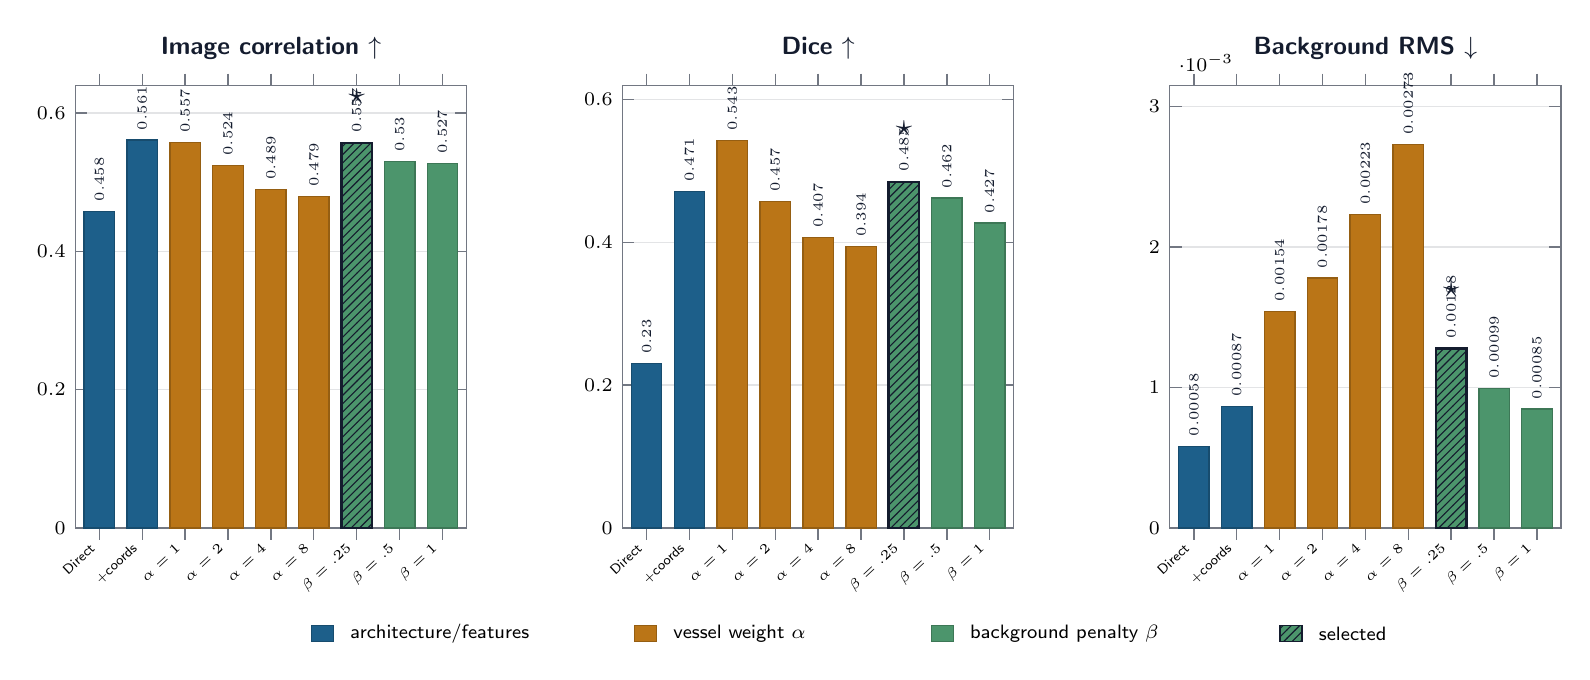
\begin{tikzpicture}
    \pgfplotsset{
      ablation panel/.style={
        width=6.55cm,
        height=7.2cm,
        ybar=0pt,
        bar width=11pt,
        bar shift=0pt,
        ymin=0,
        xtick={0,1,2,3,4,5,6,7,8},
        xticklabels={Direct,+coords,$\alpha=1$,$\alpha=2$,$\alpha=4$,$\alpha=8$,$\beta=.25$,$\beta=.5$,$\beta=1$},
        x tick label style={font=\tiny, rotate=43, anchor=east},
        tick label style={font=\scriptsize},
        title style={font=\bfseries\small, text=srlNavy},
        axis line style={draw=srlNavy!60, line width=0.5pt},
        tick style={draw=srlNavy!60, line width=0.5pt},
        ymajorgrids,
        major grid style={draw=srlNavy!12, line width=0.5pt},
        enlarge x limits=0.07,
        clip=false,
        every node near coord/.append style={font=\fontsize{4.8}{5.2}\selectfont,
          rotate=90, anchor=west, text=srlNavy},
      },
      architecture bars/.style={fill=learnedBlue, draw=learnedBlue!80!black, line width=0.5pt},
      weight bars/.style={fill=oracleAmber, draw=oracleAmber!80!black, line width=0.5pt},
      background bars/.style={fill=backgroundGreen, draw=backgroundGreen!80!black, line width=0.5pt},
      selected bar/.style={
        fill=backgroundGreen,
        draw=srlNavy,
        line width=0.9pt,
        postaction={pattern=north east lines, pattern color=srlNavy},
      },
    }

    \begin{axis}[
      ablation panel,
      at={(0cm,0cm)}, anchor=south west,
      title={Image correlation $\uparrow$},
      ymax=0.64,
      ytick={0,0.2,0.4,0.6},
      nodes near coords={\pgfmathprintnumber[fixed,precision=3]{\pgfplotspointmeta}},
    ]
      \addplot+[architecture bars] coordinates {(0,0.458) (1,0.561)};
      \addplot+[weight bars] coordinates {(2,0.557) (3,0.524) (4,0.489) (5,0.479)};
      \addplot+[selected bar] coordinates {(6,0.557)};
      \addplot+[background bars] coordinates {(7,0.530) (8,0.527)};
      \node[font=\large, text=srlNavy, anchor=south] at (axis cs:6,0.598) {$\star$};
    \end{axis}

    \begin{axis}[
      ablation panel,
      at={(6.95cm,0cm)}, anchor=south west,
      title={Dice $\uparrow$},
      ymax=0.62,
      ytick={0,0.2,0.4,0.6},
      nodes near coords={\pgfmathprintnumber[fixed,precision=3]{\pgfplotspointmeta}},
    ]
      \addplot+[architecture bars] coordinates {(0,0.230) (1,0.471)};
      \addplot+[weight bars] coordinates {(2,0.543) (3,0.457) (4,0.407) (5,0.394)};
      \addplot+[selected bar] coordinates {(6,0.485)};
      \addplot+[background bars] coordinates {(7,0.462) (8,0.427)};
      \node[font=\large, text=srlNavy, anchor=south] at (axis cs:6,0.535) {$\star$};
    \end{axis}

    \begin{axis}[
      ablation panel,
      at={(13.90cm,0cm)}, anchor=south west,
      title={Background RMS $\downarrow$},
      ymax=0.00315,
      ytick={0,0.001,0.002,0.003},
      yticklabel style={/pgf/number format/fixed,/pgf/number format/precision=3},
      nodes near coords={\pgfmathprintnumber[fixed,precision=5]{\pgfplotspointmeta}},
    ]
      \addplot+[architecture bars] coordinates {(0,0.000581) (1,0.000865)};
      \addplot+[weight bars] coordinates {(2,0.001541) (3,0.001778) (4,0.002232) (5,0.002730)};
      \addplot+[selected bar] coordinates {(6,0.001276)};
      \addplot+[background bars] coordinates {(7,0.000992) (8,0.000845)};
      \node[font=\large, text=srlNavy, anchor=south] at (axis cs:6,0.00157) {$\star$};
    \end{axis}

    \coordinate (legendCenter) at (10.15cm,-1.34cm);
    \filldraw[draw=learnedBlue!80!black,fill=learnedBlue,line width=0.5pt]
      ($(legendCenter)+(-7.15cm,-0.10cm)$) rectangle ++(0.28cm,0.20cm);
    \node[anchor=west,font=\scriptsize] at ($(legendCenter)+(-6.78cm,0)$)
      {architecture/features};
    \filldraw[draw=oracleAmber!80!black,fill=oracleAmber,line width=0.5pt]
      ($(legendCenter)+(-3.05cm,-0.10cm)$) rectangle ++(0.28cm,0.20cm);
    \node[anchor=west,font=\scriptsize] at ($(legendCenter)+(-2.68cm,0)$)
      {vessel weight $\alpha$};
    \filldraw[draw=backgroundGreen!80!black,fill=backgroundGreen,line width=0.5pt]
      ($(legendCenter)+(0.72cm,-0.10cm)$) rectangle ++(0.28cm,0.20cm);
    \node[anchor=west,font=\scriptsize] at ($(legendCenter)+(1.09cm,0)$)
      {background penalty $\beta$};
    \filldraw[
      draw=srlNavy, fill=backgroundGreen, line width=0.5pt,
      postaction={pattern=north east lines,pattern color=srlNavy}
    ] ($(legendCenter)+(5.15cm,-0.10cm)$) rectangle ++(0.28cm,0.20cm);
    \node[anchor=west,font=\scriptsize] at ($(legendCenter)+(5.52cm,0)$)
      {selected};
  \end{tikzpicture}

  \AssetCaption{Coordinates give the largest isolated gain.  Vessel weighting
  $\alpha=1$ improves localization but raises background energy; $\beta=0.25$
  is the selected balanced operating point, not the maximum of one metric.}
\end{minipage}
\end{document}
